\chapter{Fo\-bwa Language}
\section{Pronunciation of Fobwa Names}
The chart that follows is of course the Pacoitz phonology. There are other phonologies such as the Joshua phonology which is much more likely to be what the actual language sounded like. There are guides and such to the Fobwa language (the good ones use the Joshua phonology) but all that suffices for this book is a pronunciation guide (if the reader cared any more about the language, they wouldn't be reading this edition).\\
\begin{tabular}
{| l  l |}
\hline
a & \underline{u}p \\
aa & f\underline{a}ther \\
i & \underline{i}n \\
ii & f\underline{ee} \\
u & b\underline{oo} \\
e & m\underline{e}t \\
ee & m\underline{ay} \\
o & n\underline{o} \\
\hline
\end{tabular}
\begin{tabular}
{| l   l |}
\hline
w & \underline{w}ait \\
m & \underline{m}other \\
n & \underline{n}ot \\
ng & si\underline{ng} \\
p & \underline{p}ay \\
t & \underline{t}ea \\
k & \underline{c}art \\
f & \underline{f}ish \\
sh & \underline{sh}oe \\
h & \underline{h}ow \\
b & \underline{b}oat \\
d & \underline{d}og \\
g & \underline{g}o \\
v & li\underline{v}e \\
z & \underline{z}oo \\
j & sei\underline{z}ure \\
\hline
\end{tabular}
\section{Properties of Fobwa}
\label{rotshift}
Alongside \emph{The Fall of King Mwefu} original text, Pacoitz found some poems which scholars have attributed to Twizwa. And in these poems, everything that the poet says has a most peculiar property: when the page on which Twizwa's words are written is rotated 90 degrees, a second message can then be read. Not only a second though, but on subsequent rotations, a third and a fourth as well, and all of these Twizwa had carefully crafted to have the meanings line up with what he wanted to say, to not be the same thing, but to be something different that expands upon the meaning of it. They call this ``rotational shift poetry.'' This is similar to ambigrams where a word becomes a different word when read in the mirror or flipped upside down, but on a scale of paragraphs instead of just individual words. To write in Fo\-bwa in such a way is a feat in itself, for even just one rotation, but to be able to do it for all four rotations and through speech alone (as Mwefu implies in the original that Twizwa does) takes unimaginable skill. Through speech, one needs to know where the line endings are in order to visualize what the block of text will look like, that way they know what it becomes when rotated; listening to something and being able to hear all the meanings is hard, but saying it so that all the rotations are what you want them to be is even harder. When listening, the line endings will usually be where the sentence ends most commonly are. This poetry is a very very beautiful thing, but as usuall Pacoitz explains none of this and Pacoitz doesn't even make Twizwa speak in verse or say things in any way that would make it obvious. Twizwa's lack of poeticness in this version likely stems from Pacoitz's inability to write (poetry or otherwise).

\chapter{Maps}
\section{Pacoitz'}
I don't need to tell you that Pacoitz' map is worthless; there is only two place names written on the whole thing, the terrain is vague and there is only two rivers? I think Pacoitz just made this up, but he didn't even make it up based off of the places described in the text.
\begin{figure}[H]
\centering
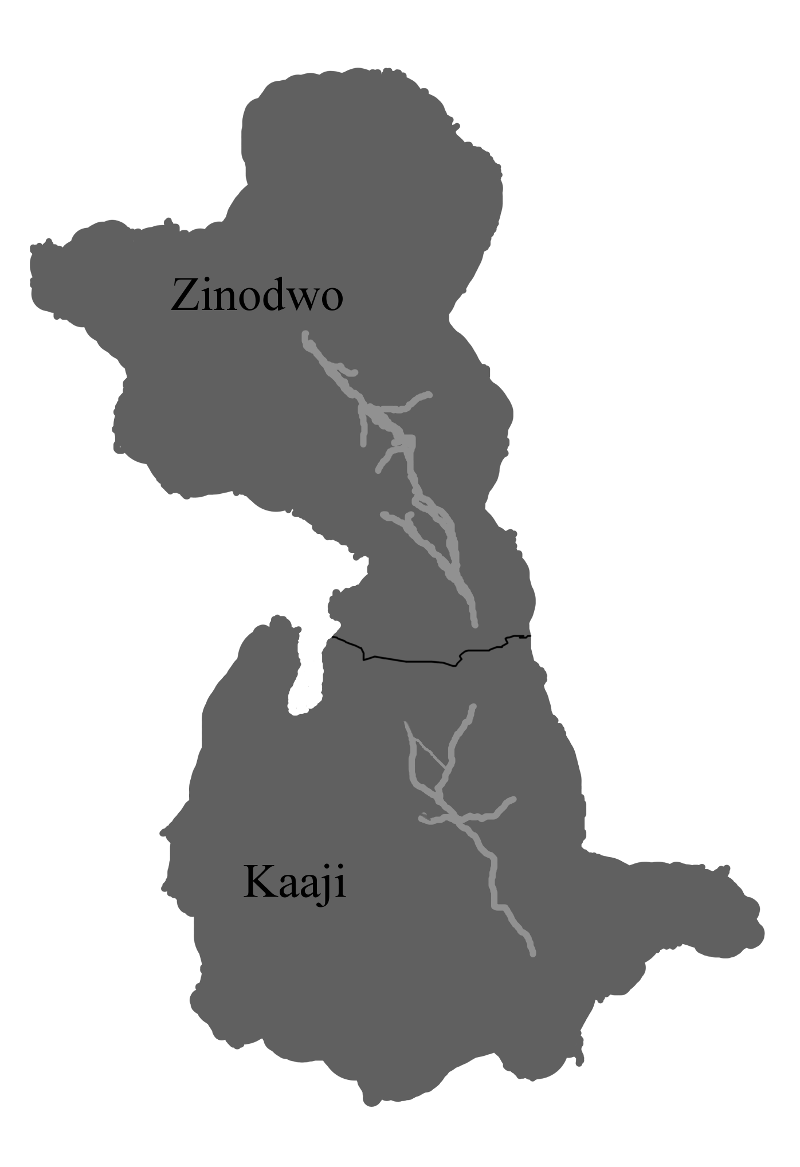
\includegraphics[width=4.5in]{Twizwa_map2.png}
\end{figure}
\clearpage

\section{Graft's}
I grew tired of looking at Pacoitz' map so I made my own using hints from the text. It's more accurate and way more informative, however, I did take some liberties.

\chapter{Origin of Fobwa Manuscripts}
In 1896, Pacoitz' worked in a restaurant located in South Dakota. But he tired of cooking and quit his job to take a vacation. (This is what Pacoitz claims, but I think it more likely that he was fired.) After a week, he found a cave in South Dakota wherein he discovered some Fobwa writing on the cave wall. Exploring further, he found some clay jars which had some poems and some historical documents as well as the original text to \emph{the Fall of King Mwefu} in them. And after working on it for a couple years he had deciphered the language.

Many found it odd that Pacoitz had discovered a language that no linguist had ever seen before and that he was able to translate it without any formal training. Now, some people have theorized that Fobwa's emergence as a language, and the fact that only Pacoitz has found any major texts in that language, proves that he fabricated the language, the narratives and other documents. I shouldn't need to tell you how ridiculous this is, but since you're reading this edition instead of another, perhaps you might need me to explain. Pacoitz is constantly mistranslating phrases from the original text as well as changing various aspects about the story; if he really had written both, then he would know how to read it and would not cut out important sections from it. If Pacoitz had written the original text, then one would expect the original to be shorter both because it was written first and also because people were only paying to read his translation because the original would be public domain since he claimed that someone else wrote it hundreds of years prior.

Pacoitz is just not creative enough to come up with anything original, let alone create an elaborate well-thought-out hoax to purport a translation of what would be fake documents written in a fake language.

Not a single scholar of any standing finds any of \emph{the Elevated Pacoitz Doctrine} (As some call it) to have even an inkling of credibility. The texts have all the evidence of older productions; Joshua Greenberg confirmed the works (via carbon dating some excess paper) to be at least 1,300 years old. So it is highly probable that Fobwa, and \emph{The Fall of King Mwefu} are historical works and not apocryphal.

\chapter{Omitted Plot}
\emph{Whinery Press} does not have any other translations of \emph{The Fall of King Mwefu} licensed for use in this book, so I have paraphrased the parts of the story which the reader has been deprived of because Pacoitz left them out.

\section{The Foreigner and His Wife}
\label{foreigner1}

(Before King Mwefu leaves to return to his raid in Zinodwo, he is summoned to deal with some unwanted immigrants -- a man and a wife.)

``How did you get in here?'' I Asked.

``We walked in.'' Said the man; his speech was very stilted and regular and it was obvious that he was a foreigner.\footnote{Fobwa is a very hard language to learn. The irregularity in the word order (and the words are small and many are needed) is borderline unnatural.}

``What do you want?'' I Said, rather annoyed.

``To tell you the good news.'' Replied the wife also poorly.

``You're here to pay tribute?'' I asked.

``No, if your soul could have been bought with silver it would have been already by now.'' The man said this, and had become eloquent somehow in contrast to how he spoke before, ``The one true god wanted to be our friend, but none of us could because of all the evil that we do, the evil that we are from birth. So he --''

``Oh really? We are enlightened.'' I Said, ``We know that there are no gods. For if there were, they would have protected Kaaji from my armies. But they're nothing but wood and stone. And you call me evil? I protect my country, I share my wealth!'' And with that I had the two foreigners imprisoned and tortured. The couple took their punishment with remarkable patience; but after awhile, the tormentors tired of inflicting such travail and rested. On seeing their resolve, I let the foreigners go, but would not speak with them.
